\subsection{Images}
\label{sec:images}

Next, we study images in terms of their popularity, size and their use of layers.

\begin{figure}[!t]
	\centering
	\subfigure[CDF of repositories by pull count]{\label{fig_pull_cnt_total}
		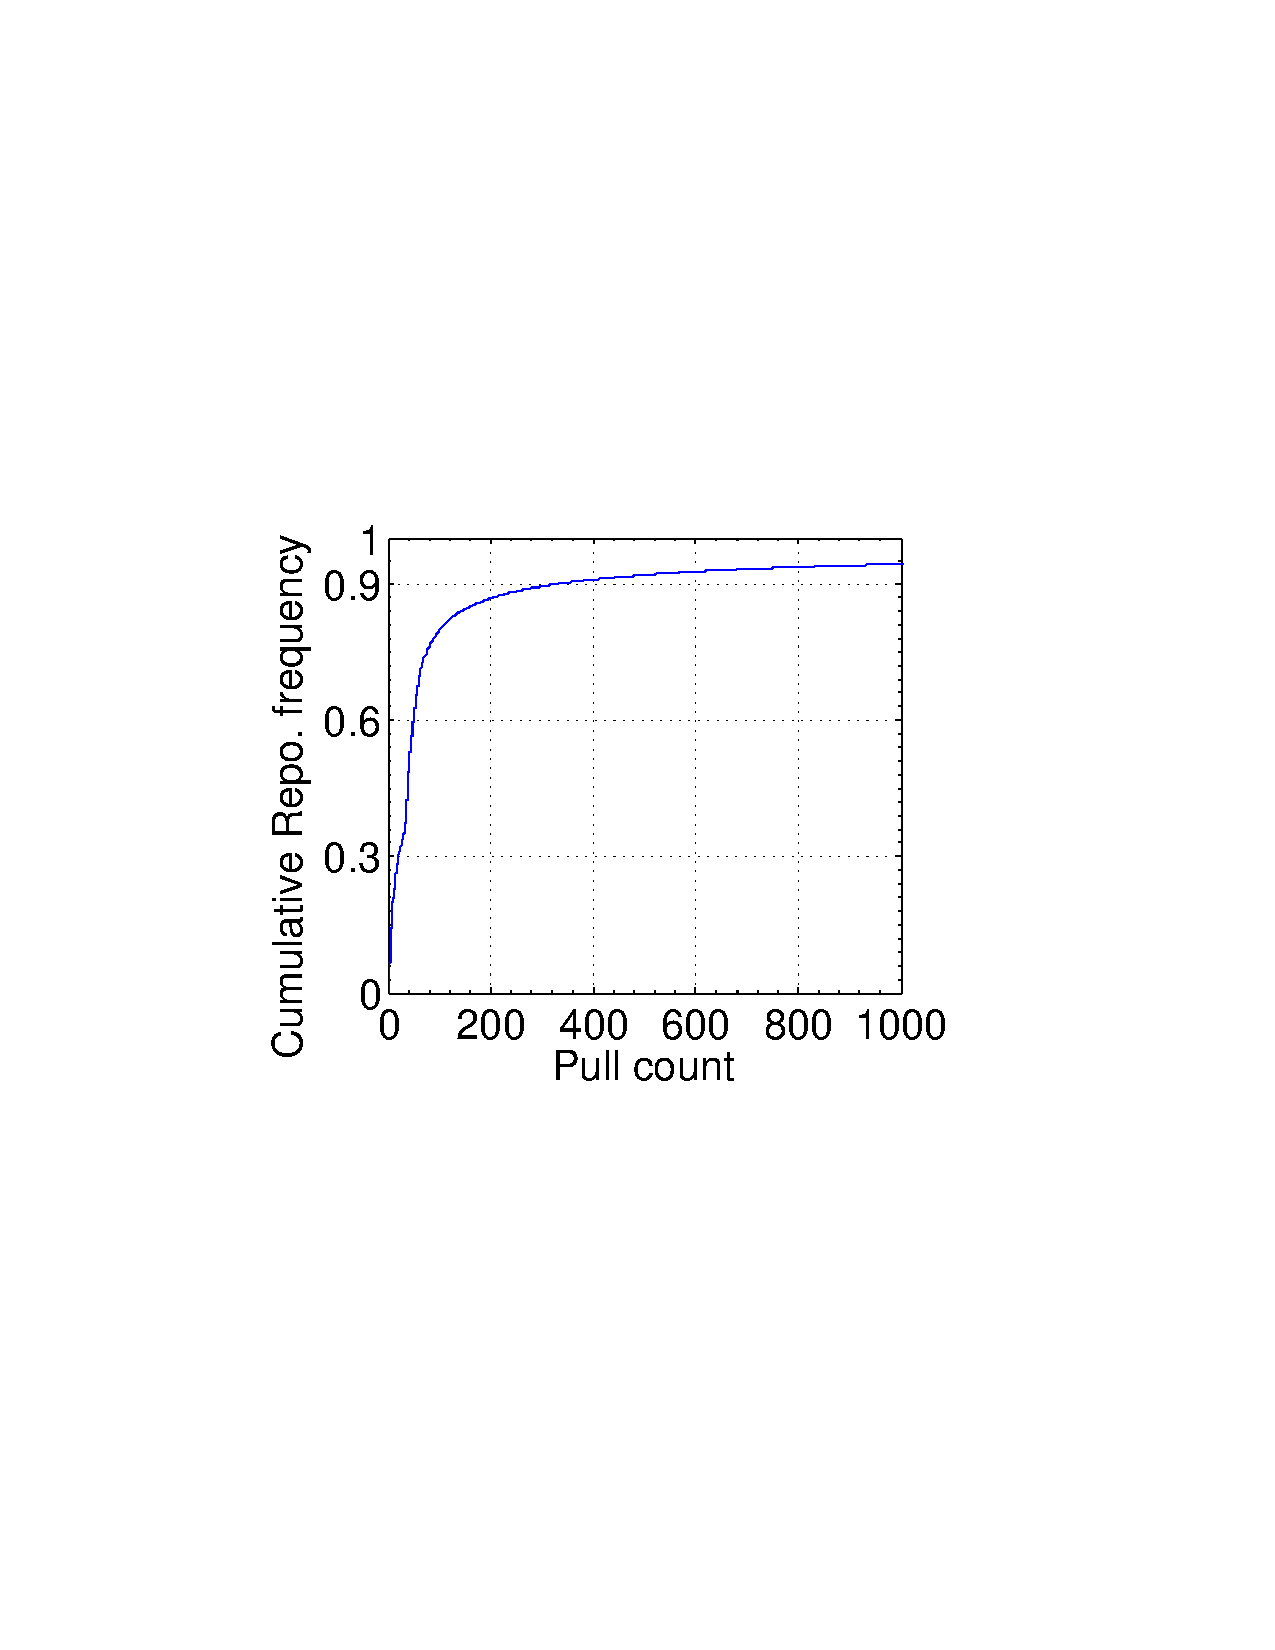
\includegraphics[width=0.23\textwidth]{graphs/pull_cnt.pdf}
	}
	\subfigure[Histogram of repositories by pull count]{\label{fig_pull_cnt_count}
		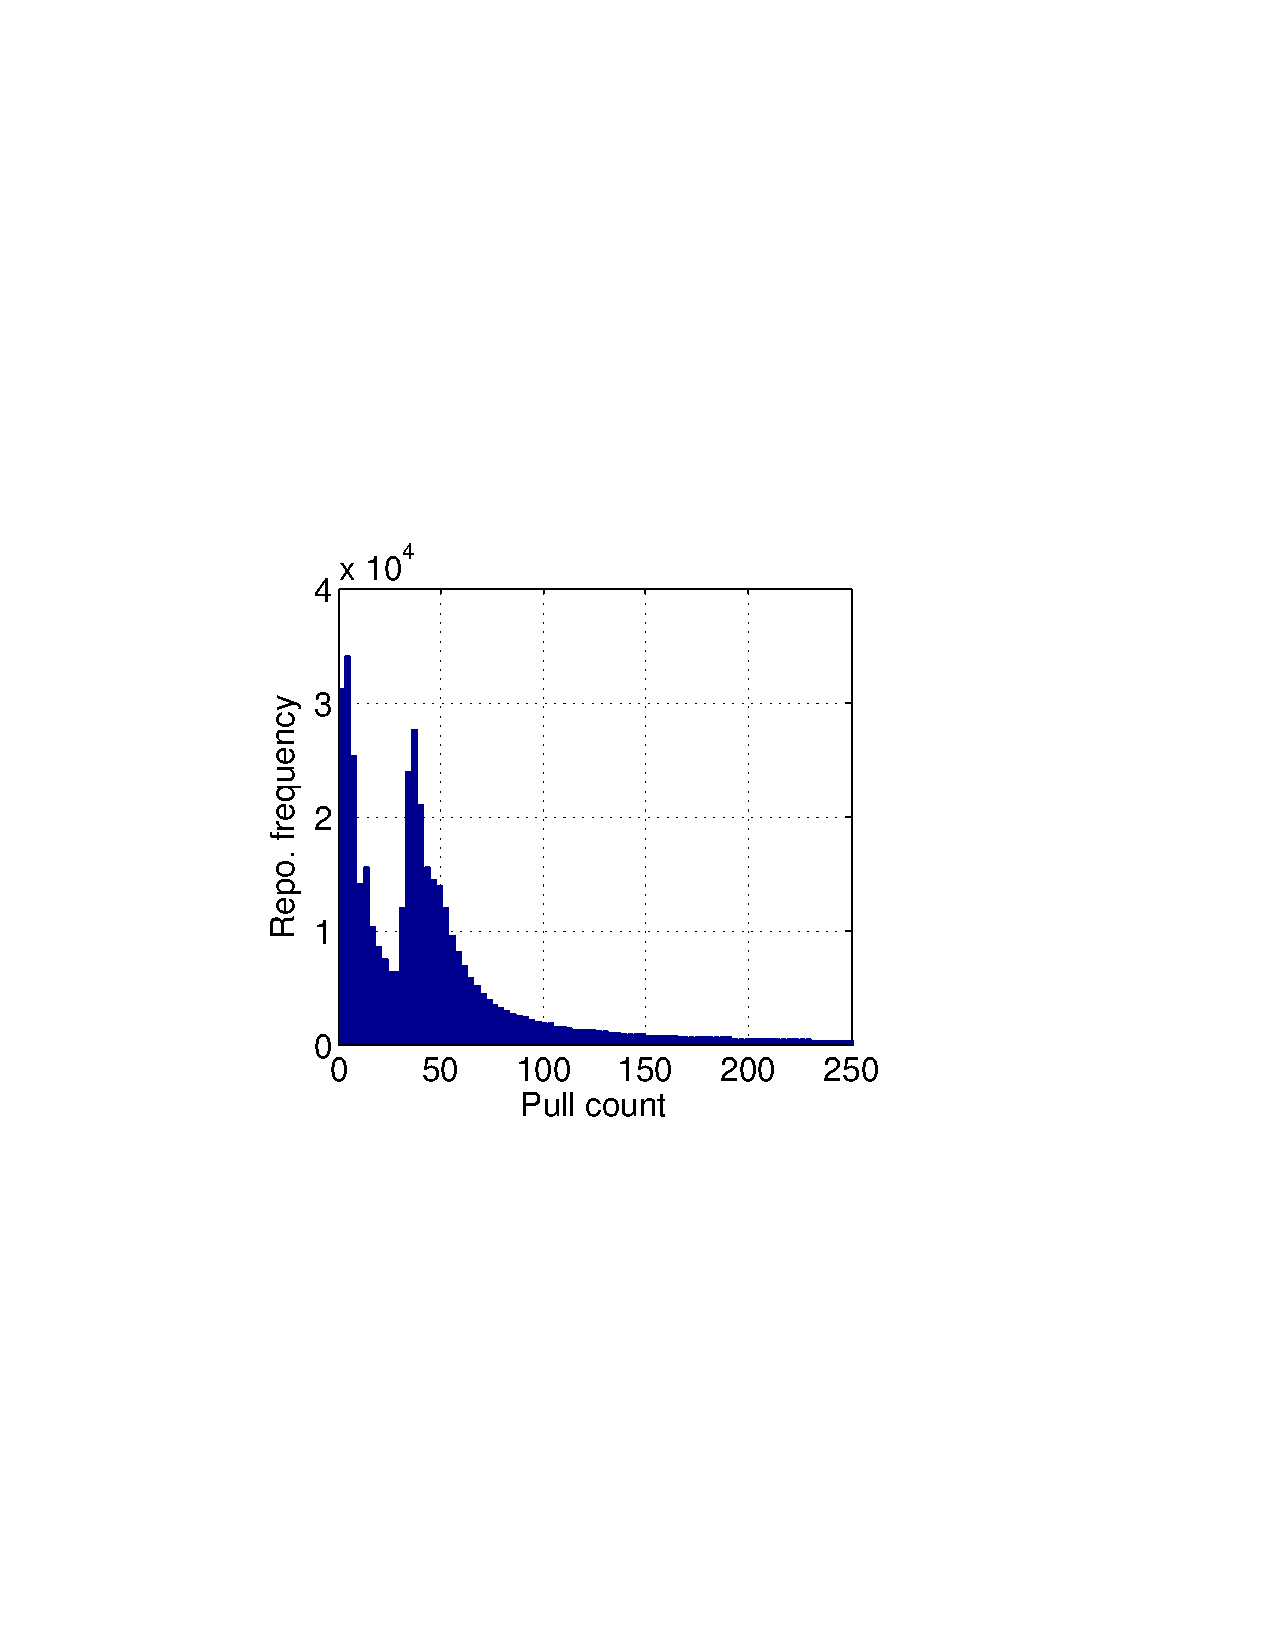
\includegraphics[width=0.22\textwidth]{graphs/count_pull_cnt.pdf}
	}
	\caption{Repository popularity distribution}
	\label{fig-pop}
\end{figure}

\paragraph{Image popularity}
%
We start by analyzing image popularity.
Figure~\ref{fig-pop} shows the repository popularity distribution on May 31st in
terms of the pull count of individual images.
%The x-axies show the pull count (i.e., total number of pulls) for repositories
%by May 31th with different ranges.  
The CDF in Figure~\ref{fig_pull_cnt_total} reveals a large degree of skew in image
pulls. In the median, images are only pulled 40 times while in the 90\% percentile we
see a pull count of 333. On the other hand, the largest pull count is more than 650M 
which is for the official \textit{nginx} repository. This is followed by
Google's \textit{cadvisor} (434M pulls), \textit{redis} (264M pulls),
\textit{ubuntu} (28M pulls) and GliderLabs' \textit{registrator} (212M pulls).


Looking at the pull frequencies for repositories (see Figure~\ref{fig_pull_cnt_count})
confirms the skewness. We see that 31,200 of repositories are only pulled between 0 and
2 times while 34,100 repositories are pulled between 3 to 5 times. What is interesting is
that there is a second peak around a pull count of 37 which does not fit a heavy-tailed
distribution.
%\lrcomment{Any explanation for this?}

%and 27,600 repositories are pulled
%~37 times, which are the two peaks shown in the figure.  Overall, repository
%frequency decreases with the pull count.

The skewness of two curves in Figure~\ref{fig-pop} suggests that Docker hub is
a good fit for caching popular repositories or images to
reduce \textit{pull} latencies.

%%%%%%%%%%%%%%%%%%%%%%%%%%%%%%%%%%%%%%%%%%%%%%%%%%%%%%%%%%%%%%%%%%%%%

\paragraph{Image size distribution}
\label{sec:image-size}


\begin{figure}[!t]
	\centering
	\subfigure[CDF of images by size (GB)]{\label{fig_image_size_gb}
		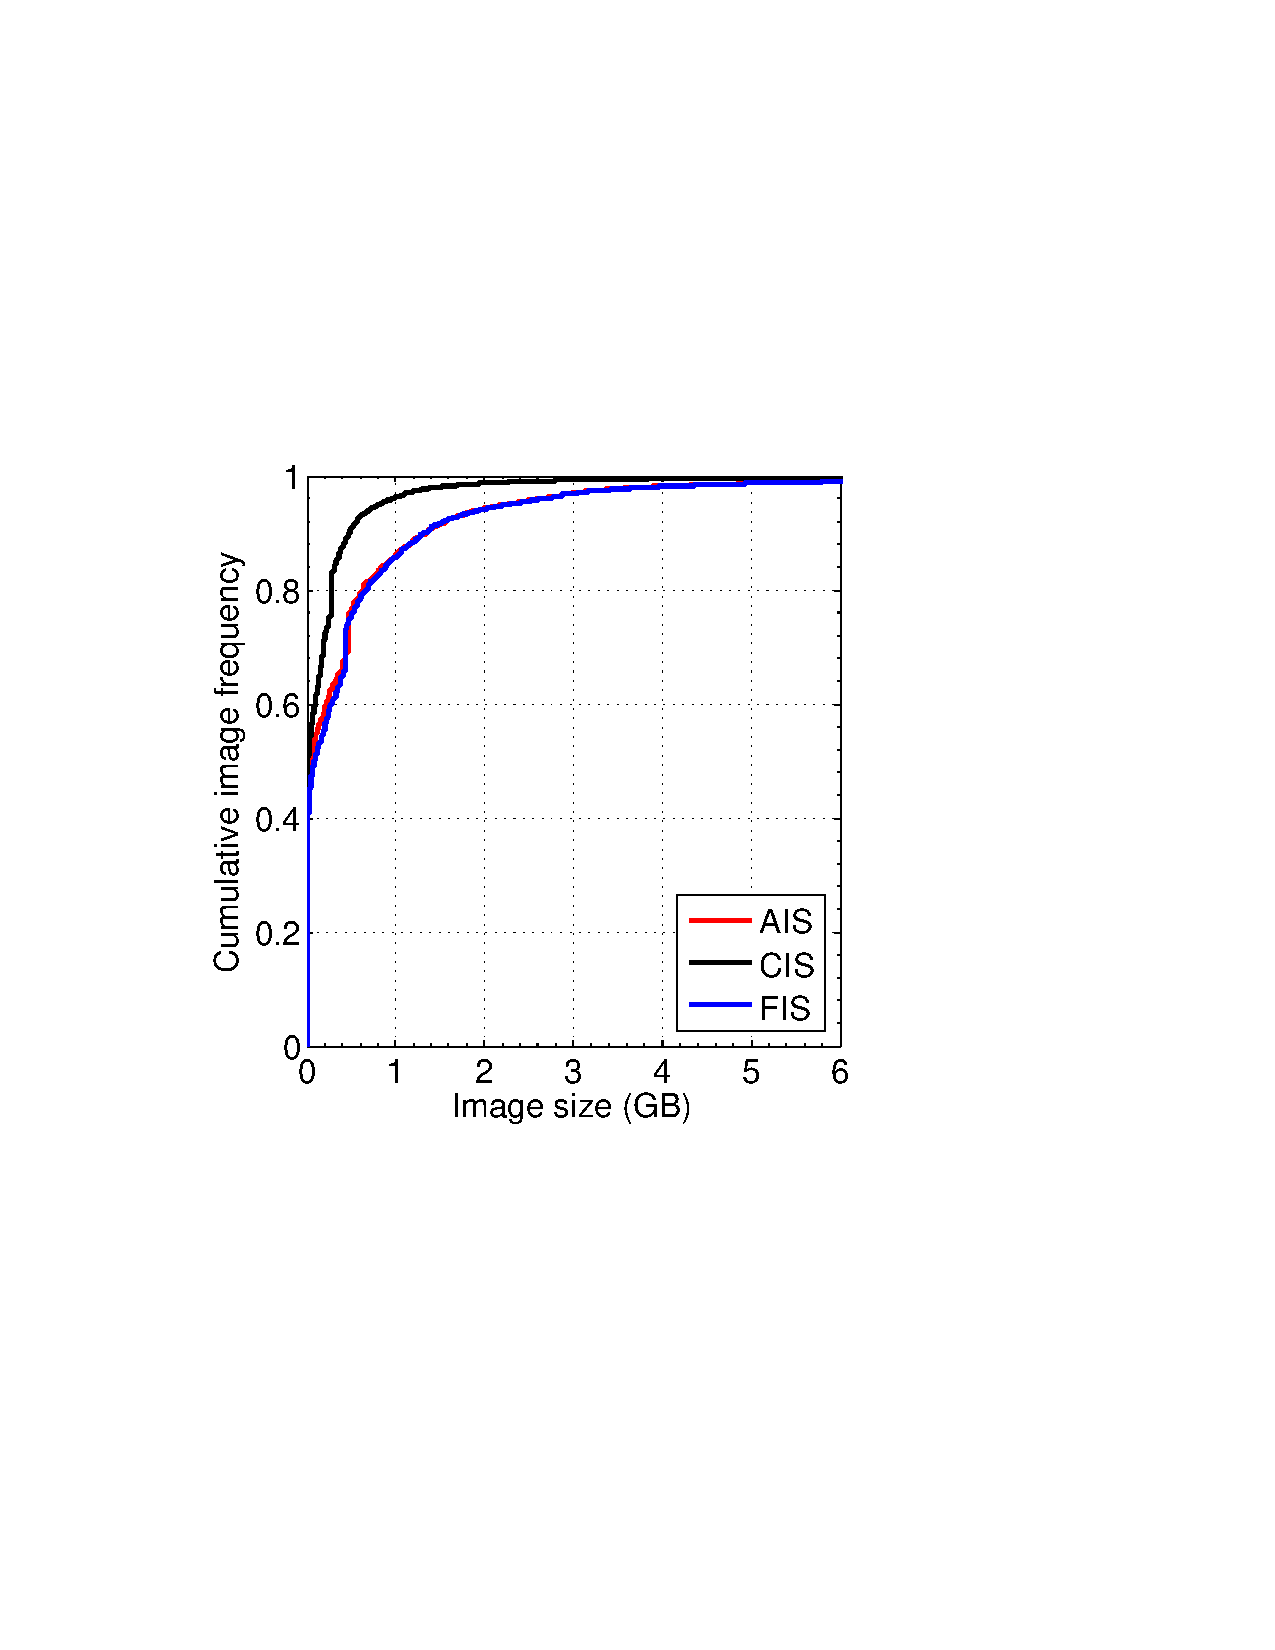
\includegraphics[width=0.22\textwidth]{graphs/size.pdf}
	}
	\subfigure[CDF of images by size (MB)]{\label{fig_image_size_mb}
		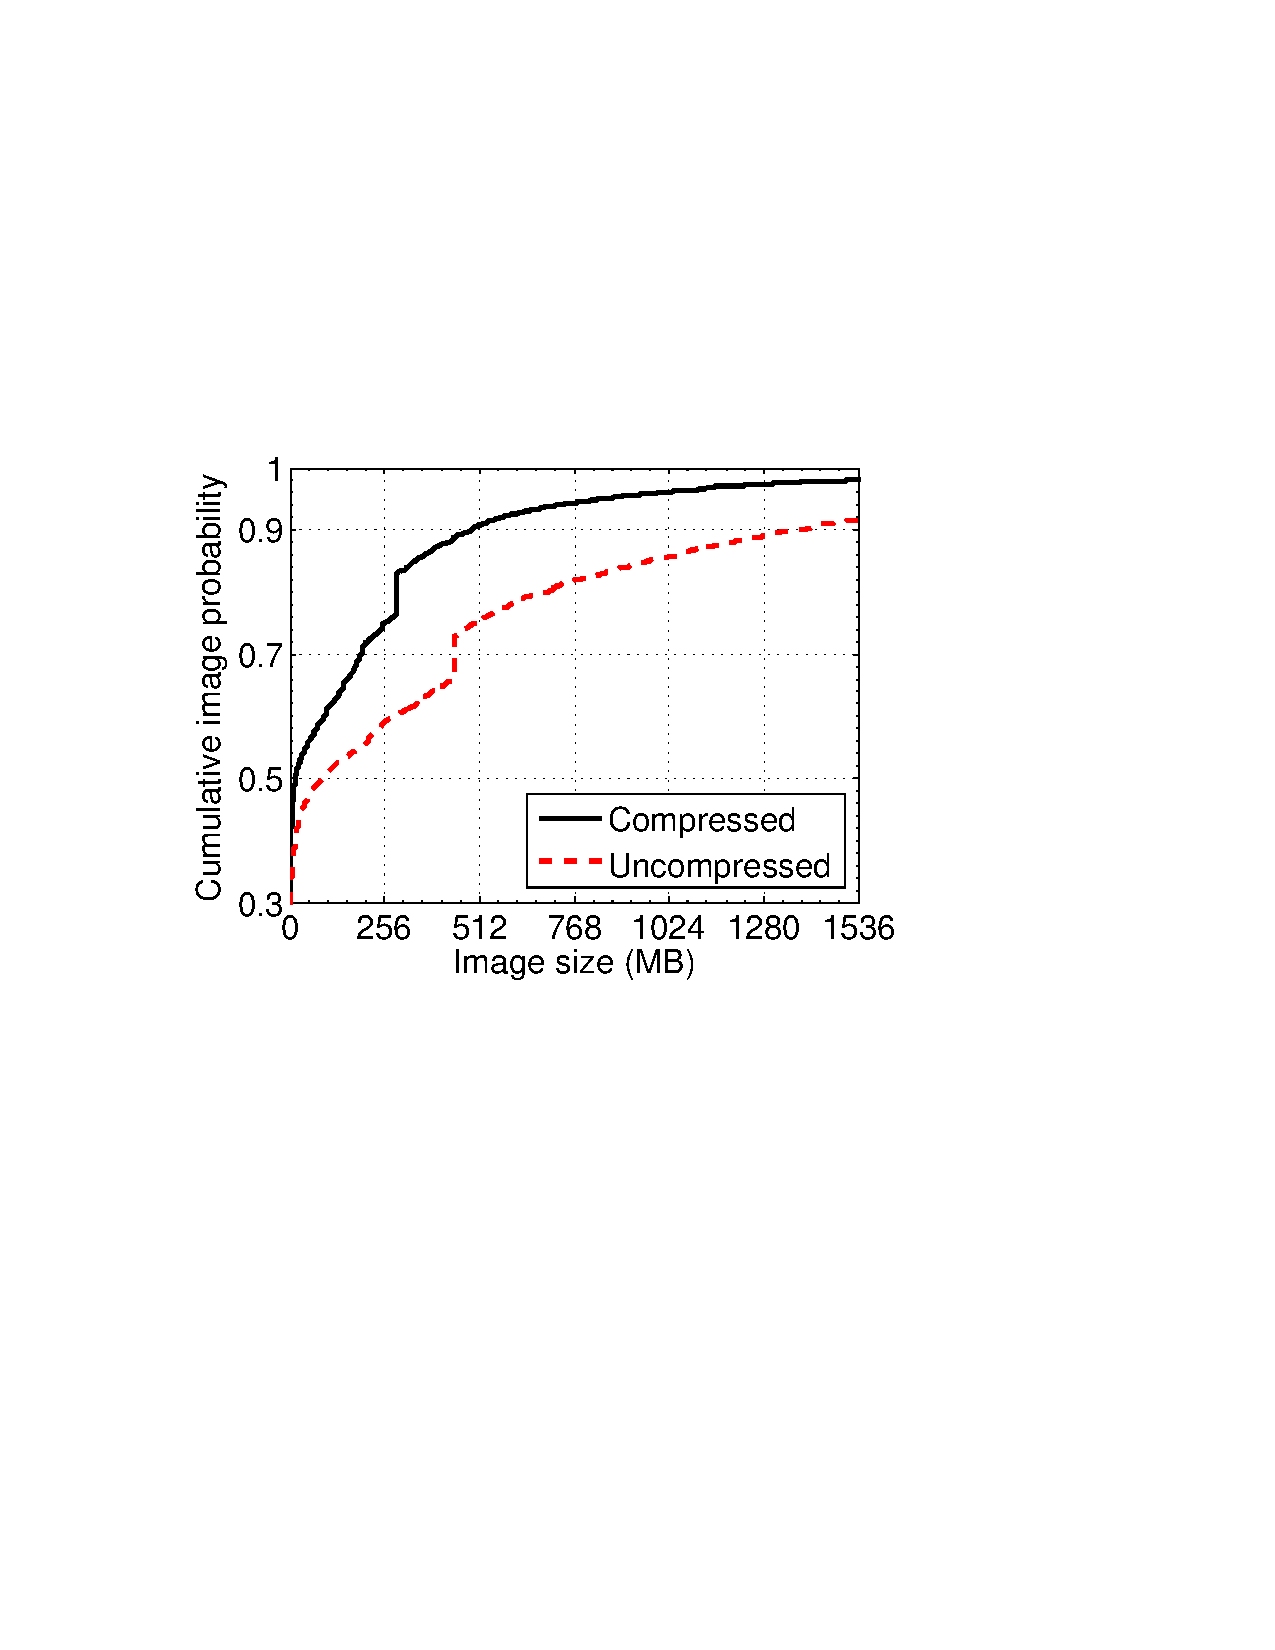
\includegraphics[width=0.23\textwidth]{graphs/size_mb.pdf}
	}
	\caption{Image size distribution}
	\label{fig-image-size}
\end{figure}


\begin{figure}[!t]
	\centering
	\subfigure[CDF of layer count in images]{\label{fig_layer_cnt_less}
		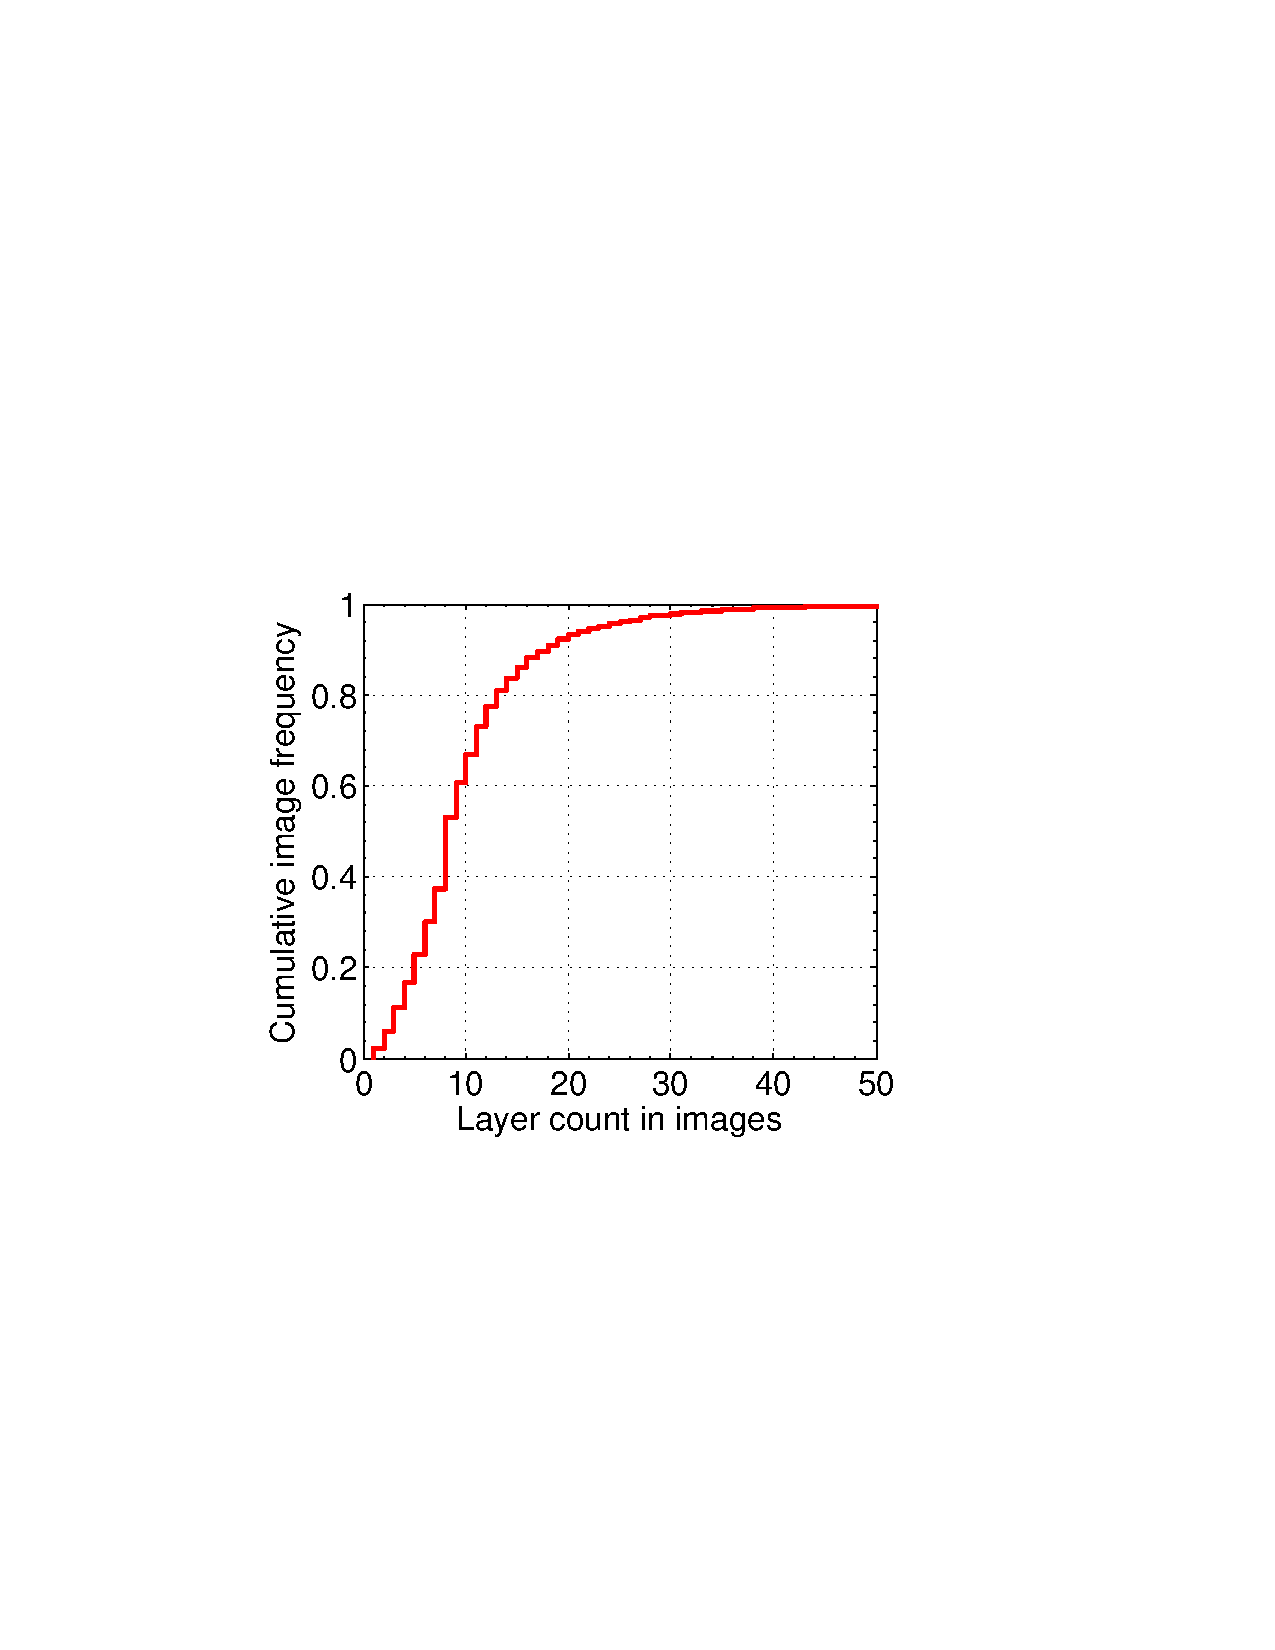
\includegraphics[width=0.23\textwidth]{graphs/layer_cnt_less.pdf}
	}
	\subfigure[Histogram of layer count in images]{\label{fig_hist_layer_cnt}
		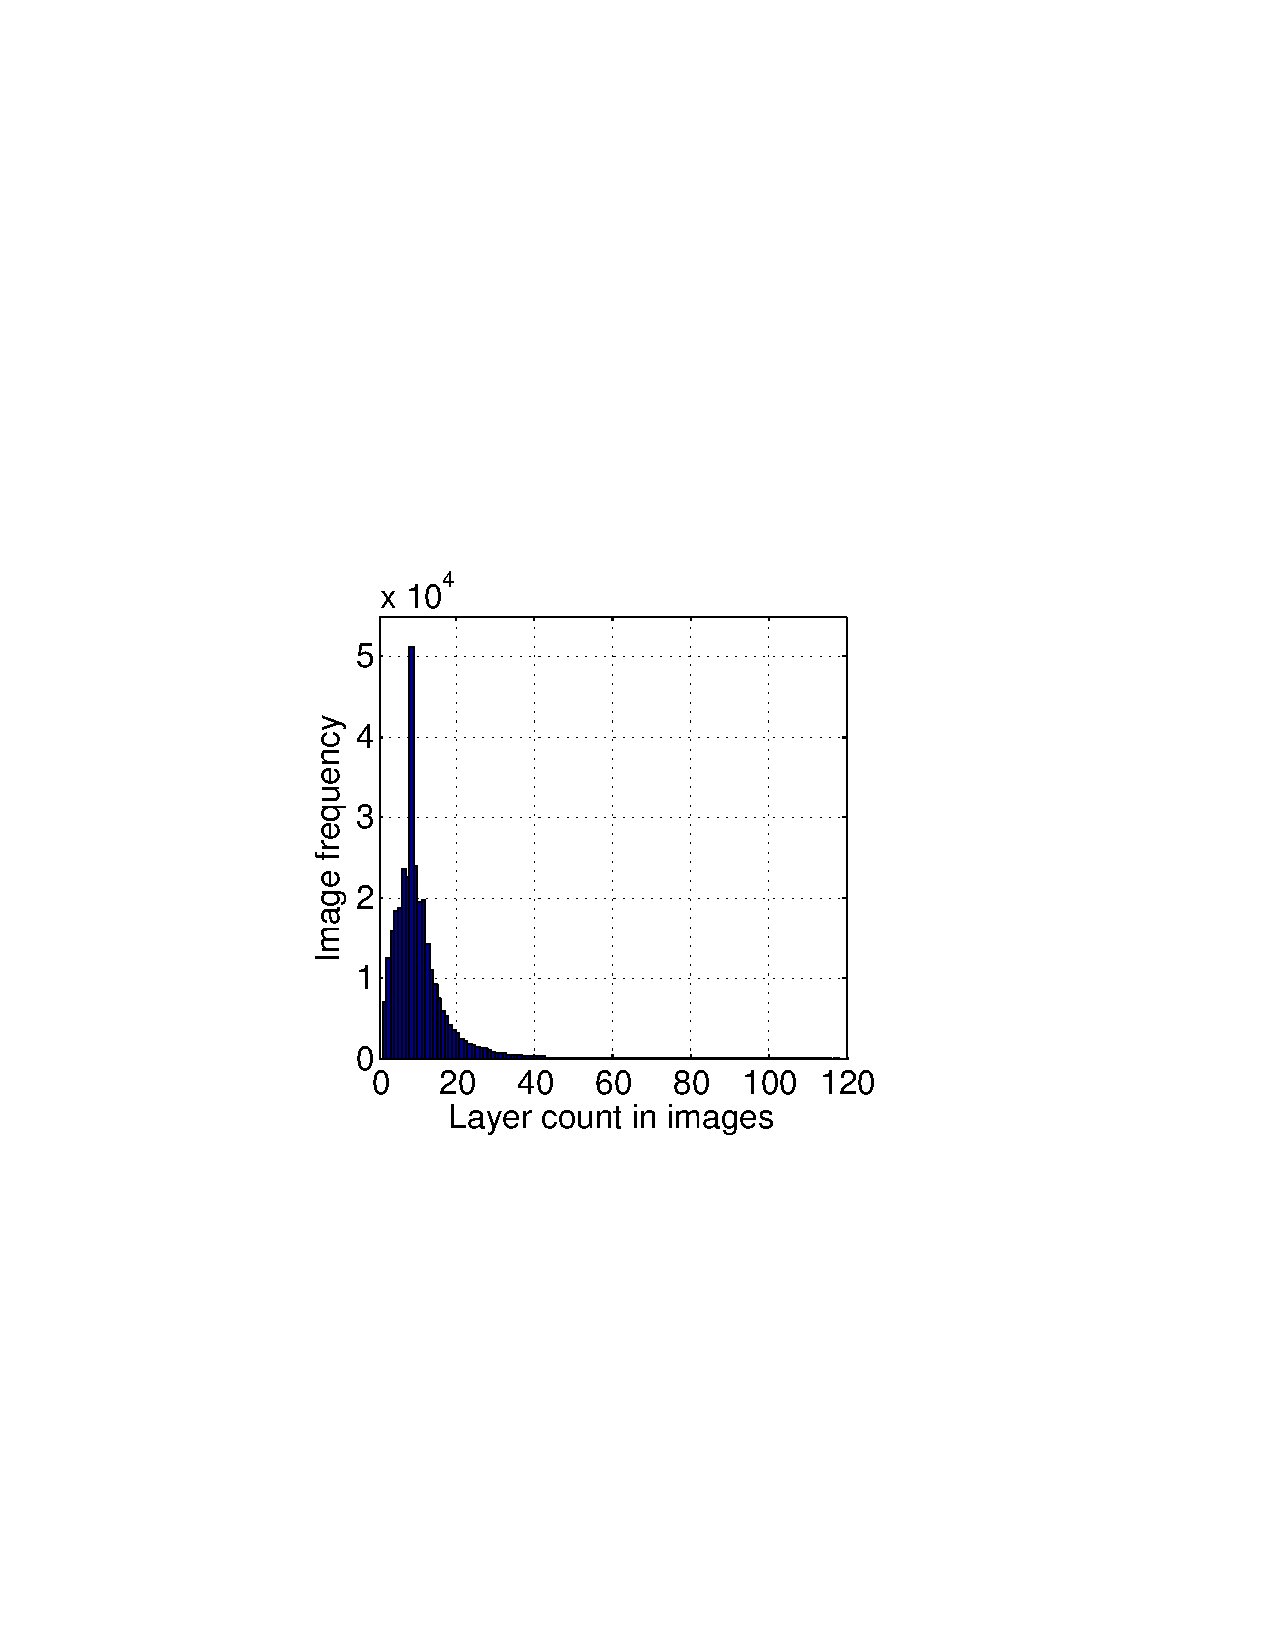
\includegraphics[width=0.213\textwidth]{graphs/hist_layer_cnt.pdf}
	}
	\caption{Layer count}
	\label{fig-layer-cnt}
\end{figure}

Similarly to layers, we also measure compressed image size
(CIS), \ie the sum of the sizes of the compressed image layers, and the sum of the
sizes of files contained in the image (FIS). Figure~\ref{fig_image_size_gb}
and~\ref{fig_image_size_mb} show the image size distributions at a coarse GB resolution
and a finer resolution only covering images smaller than 1.5 GB.

90\% of the images have an uncompressed size less than 1.3 GB while compressed images
are less than 0.48 GB. In the median, this decreases to 94MB and 17 MB, respectively.
The largest uncompressed image is 498 GB which is a Ubuntu-based image.
Figure~\ref{fig-image-size} shows that the majority of uncompressed images in Docker Hub are
small which aligns with the Docker philosophy to package software and distribute
software in containers but include only its necessary dependencies.

%As shown in figure~\ref{fig_image_size_gb}, The CDF distribution of images for AIS and FIS are
%almost similar. 90\% of images have a less than 1.3GB decompressed size for either FIS or AIS,
%while 90\% of images can be compressed less than 0.48 GB. The largest AIS and FIS are ~498 GB
%while the largest CIS is only 202 GB.

%Figure~\ref{fig_image_size_mb} shows the cumulative image probability by image size in MBs.
%70\% of the images can be compressed less than 190 MB. And 70\% of the images have a less
%than 478 MB uncompressed size (i.e., AIS or FIS). Half of the images can be compressed less
%than ~17 MB. Half of the images are less than 46 MB in AIS format and 94 MB in FIS formats
%respectively.

%\paragraph{Compression rate distribution}
%
%\begin{figure}[!t]
	\centering
	\subfigure[CDF of images by compression ratio]{\label{fig_image_compression_ratio}
		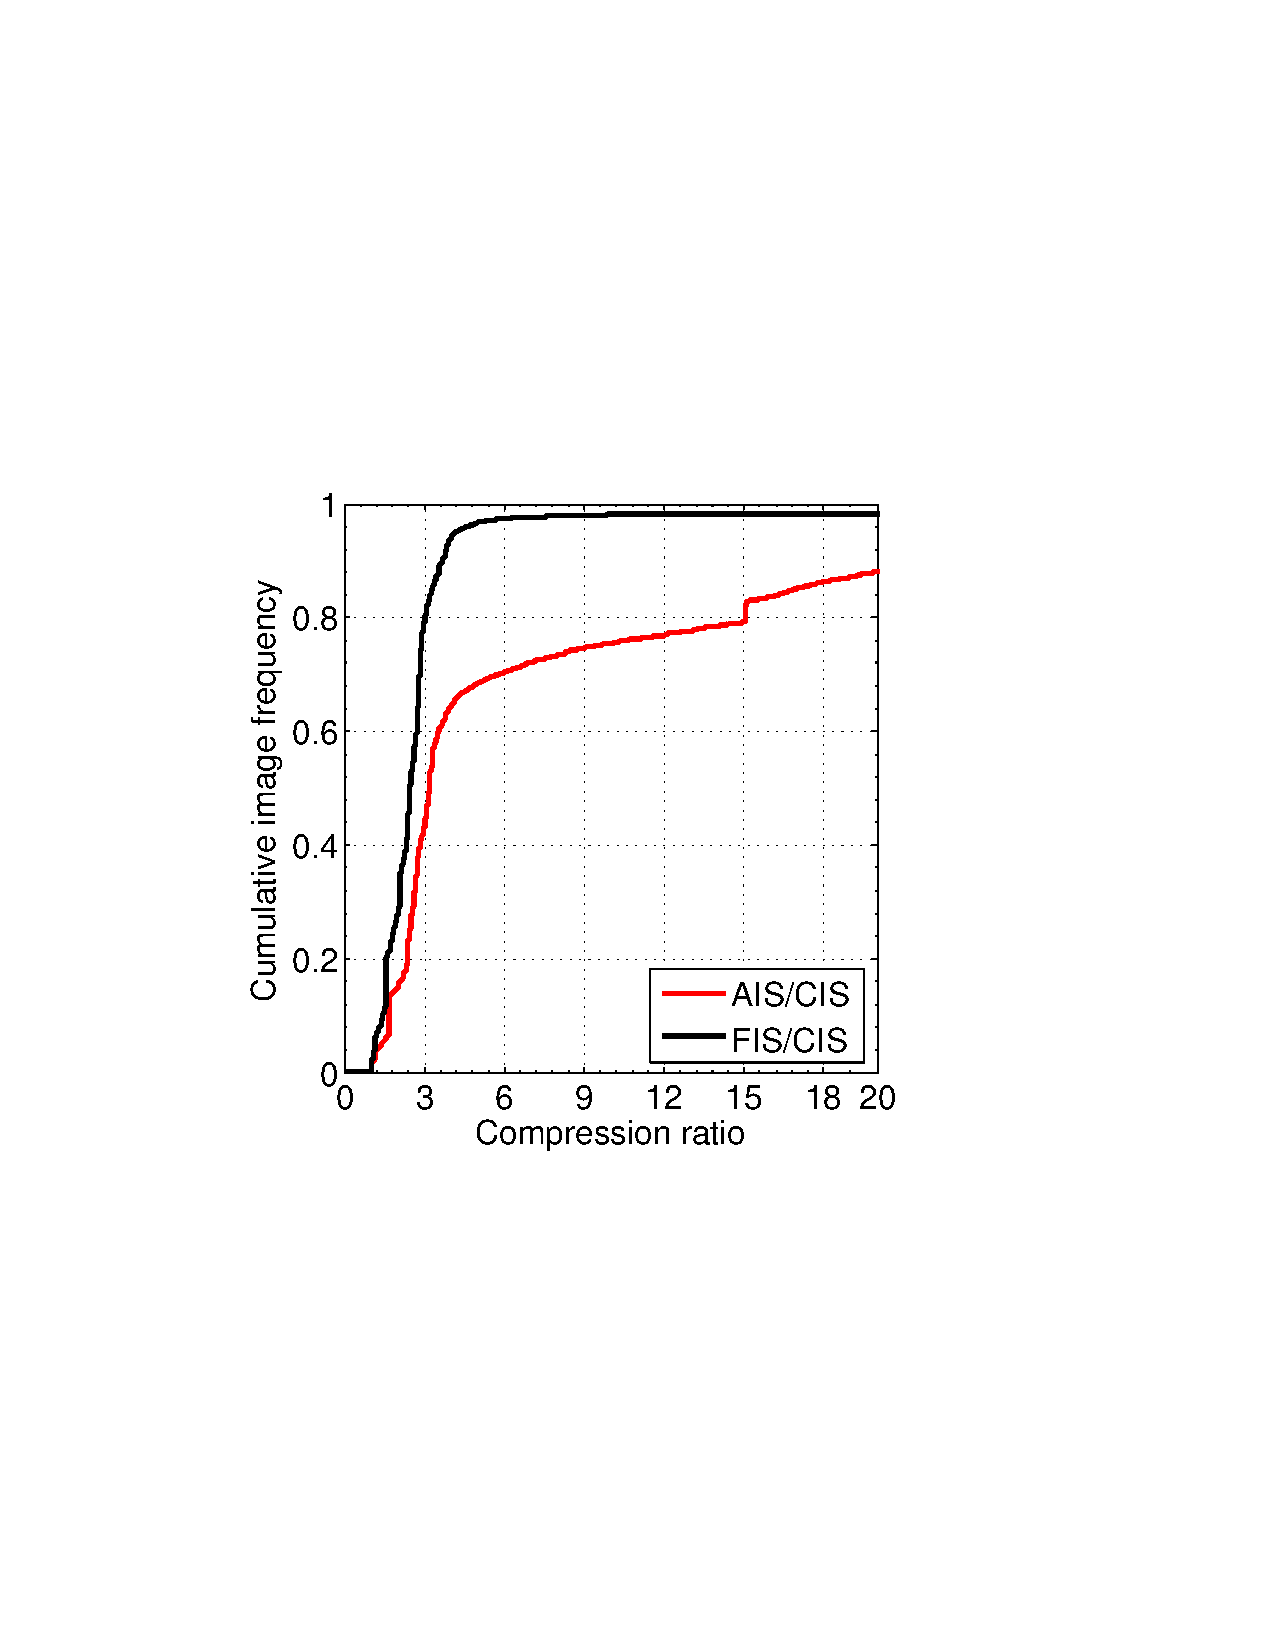
\includegraphics[width=0.23\textwidth]{graphs/compression_ratio_less.pdf}
	}
	\subfigure[Histogram of images by compression ratio]{\label{fig_image_compression_ratio_less}
		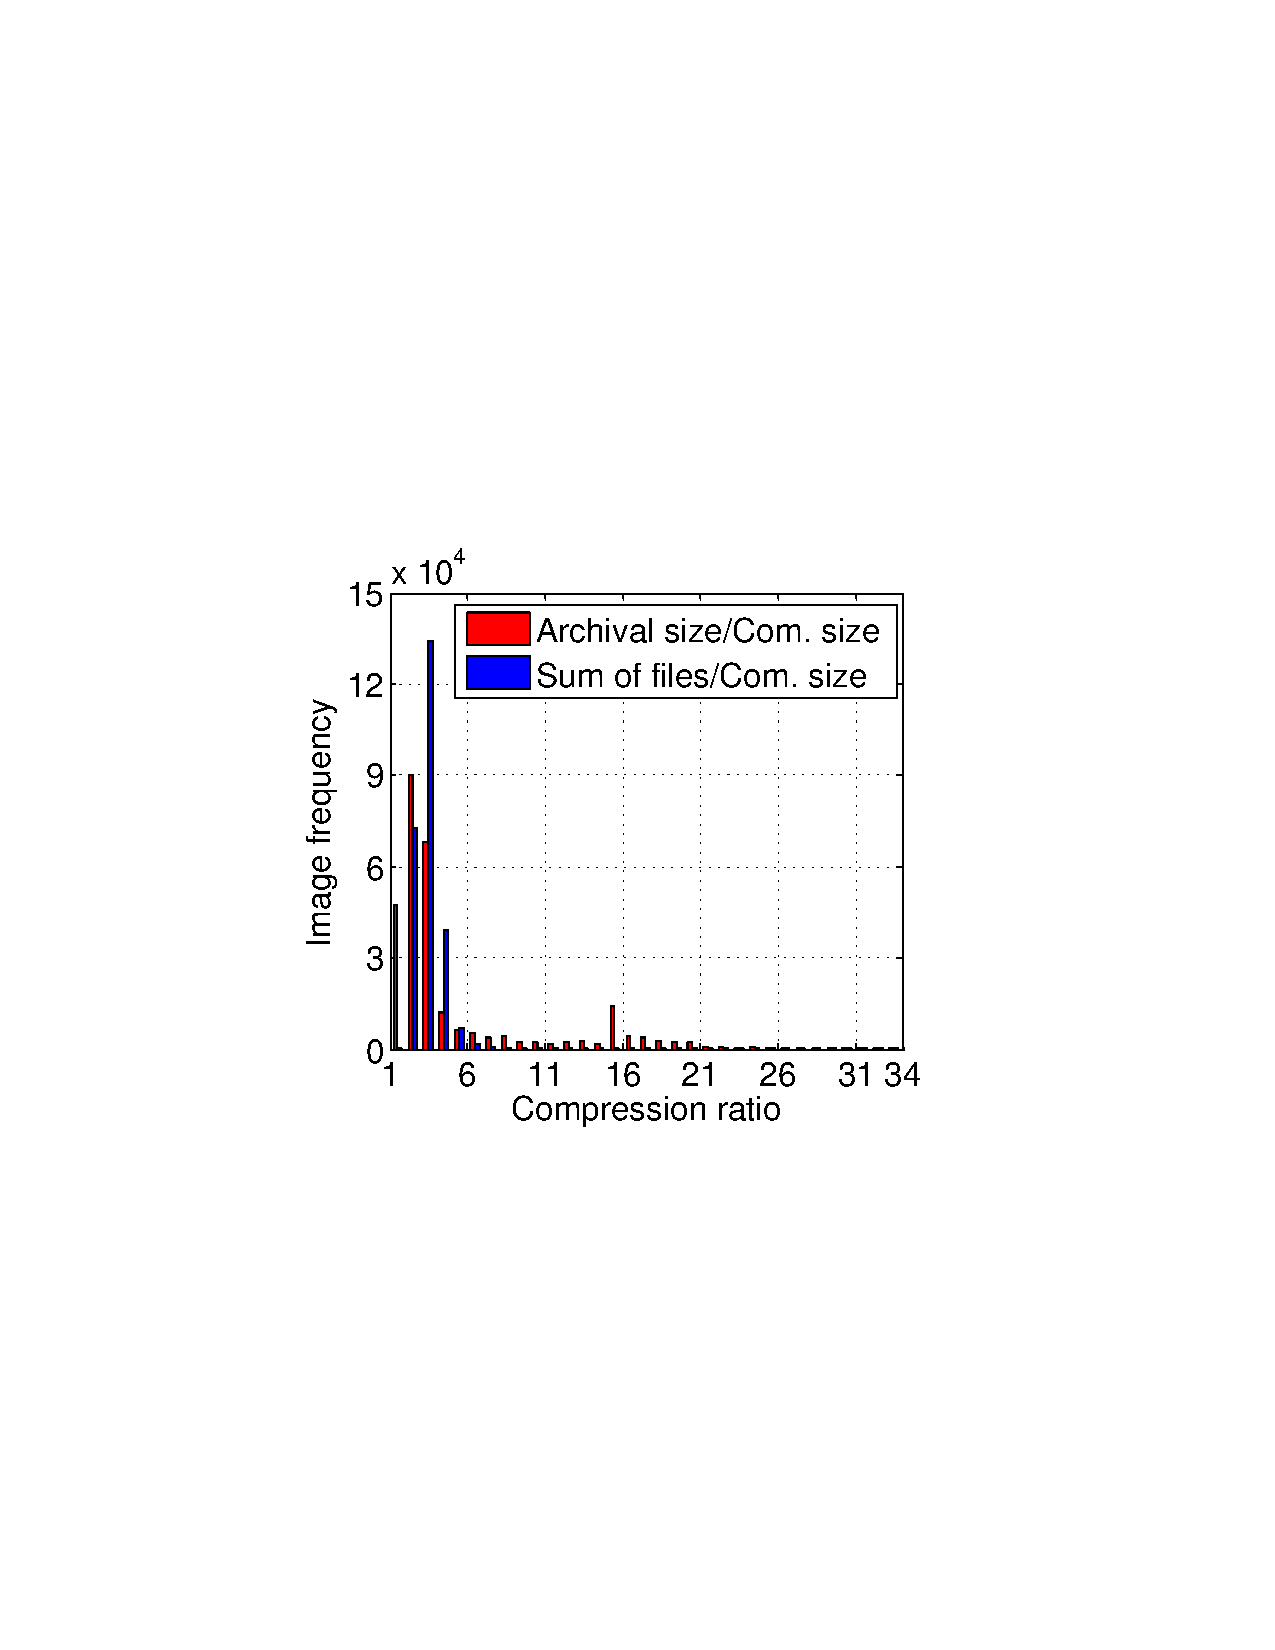
\includegraphics[width=0.223\textwidth]{graphs/hist_compression_ratio.pdf}
	}
	\caption{Compression rate distribution}
	\label{fig-image-compression-ratio}
\end{figure}
%
%To understand compressibility, we again compute the FIS-to-CIS compression ratio
%
%%As discussed in~\ref{sec:image-size}, three kinds of image size are measured: AIS, CIS, and
%%FIS. Thus, we calculated two kinds of compression ratio: the ratio of AIS to CIS (AIS-to-CIS)
%%and the ratio of FIS to CIS (FIS-to-CIS).
%
%Figure~\ref{fig-image-compression-ratio} shows the cumulative image probability by compression
%ratio. Overall, we can see that AIS-to-CIS is greater than FIS-to-CIS. 90\% of images have a
%AIS-to-CIS less than ~4 while 90\% of images have a FIS-to-CIS less than 35. Half of the images
%have a compression ratio (both AIS-to-CIS and FIS-to-CIS) around 3. The maximum compression
%ratio are 512,930 and 1028 in FIS-CIS and AIS-CIS formats respectively.
%Figure~\ref{fig_image_compression_ratio_less} shows a histogram of image probability by
%compression ratio. 134,000 images' FIS-to-CISs are 3.5 and 90,000 images'AIS-to-CISs are 2.5,
%which are two peaks shown in the graph.
%
%Figure~\ref{fig-image-compression-ratio} suggests that Docker images has a great potential
%for compression to save space.

%%%%%%%%%%%%%%%%%%%%%%%%%%%%%%%%%%%%%%%%%%%%%%%%%%%%%%%%%%%%%%%%%%%%%


\paragraph{Layer count distribution}

As discussed in~\ref{sec-image-layers}, images consist of a set of layers.
It is important to understand the layer count of the images as previous
work found that the number of layers can impact the performance of
I/O operations~\cite{slacker}. Therefore, we count the number of layers
per image and plot the CDF (see Figure~\ref{fig-layer-cnt})
and layer count frequencies (see Figure~\ref{fig_hist_layer_cnt})for all
Docker Hub images.

The results show that 90\% of the images have less than 18 layers while
half of the images have less than 8 layers. 8 layers is also the most
frequent layer value with 51,300 images consisting of exactly 8 layers.
The maximum layer count is 120 in the \textit{cfgarden/120-layer-image}.
We also find that there are 7,060 images which only consist of a single layer.

\begin{figure}[!t]
	\centering
	\subfigure[CDF of layer reference count]{\label{fig_repeate_layer}
		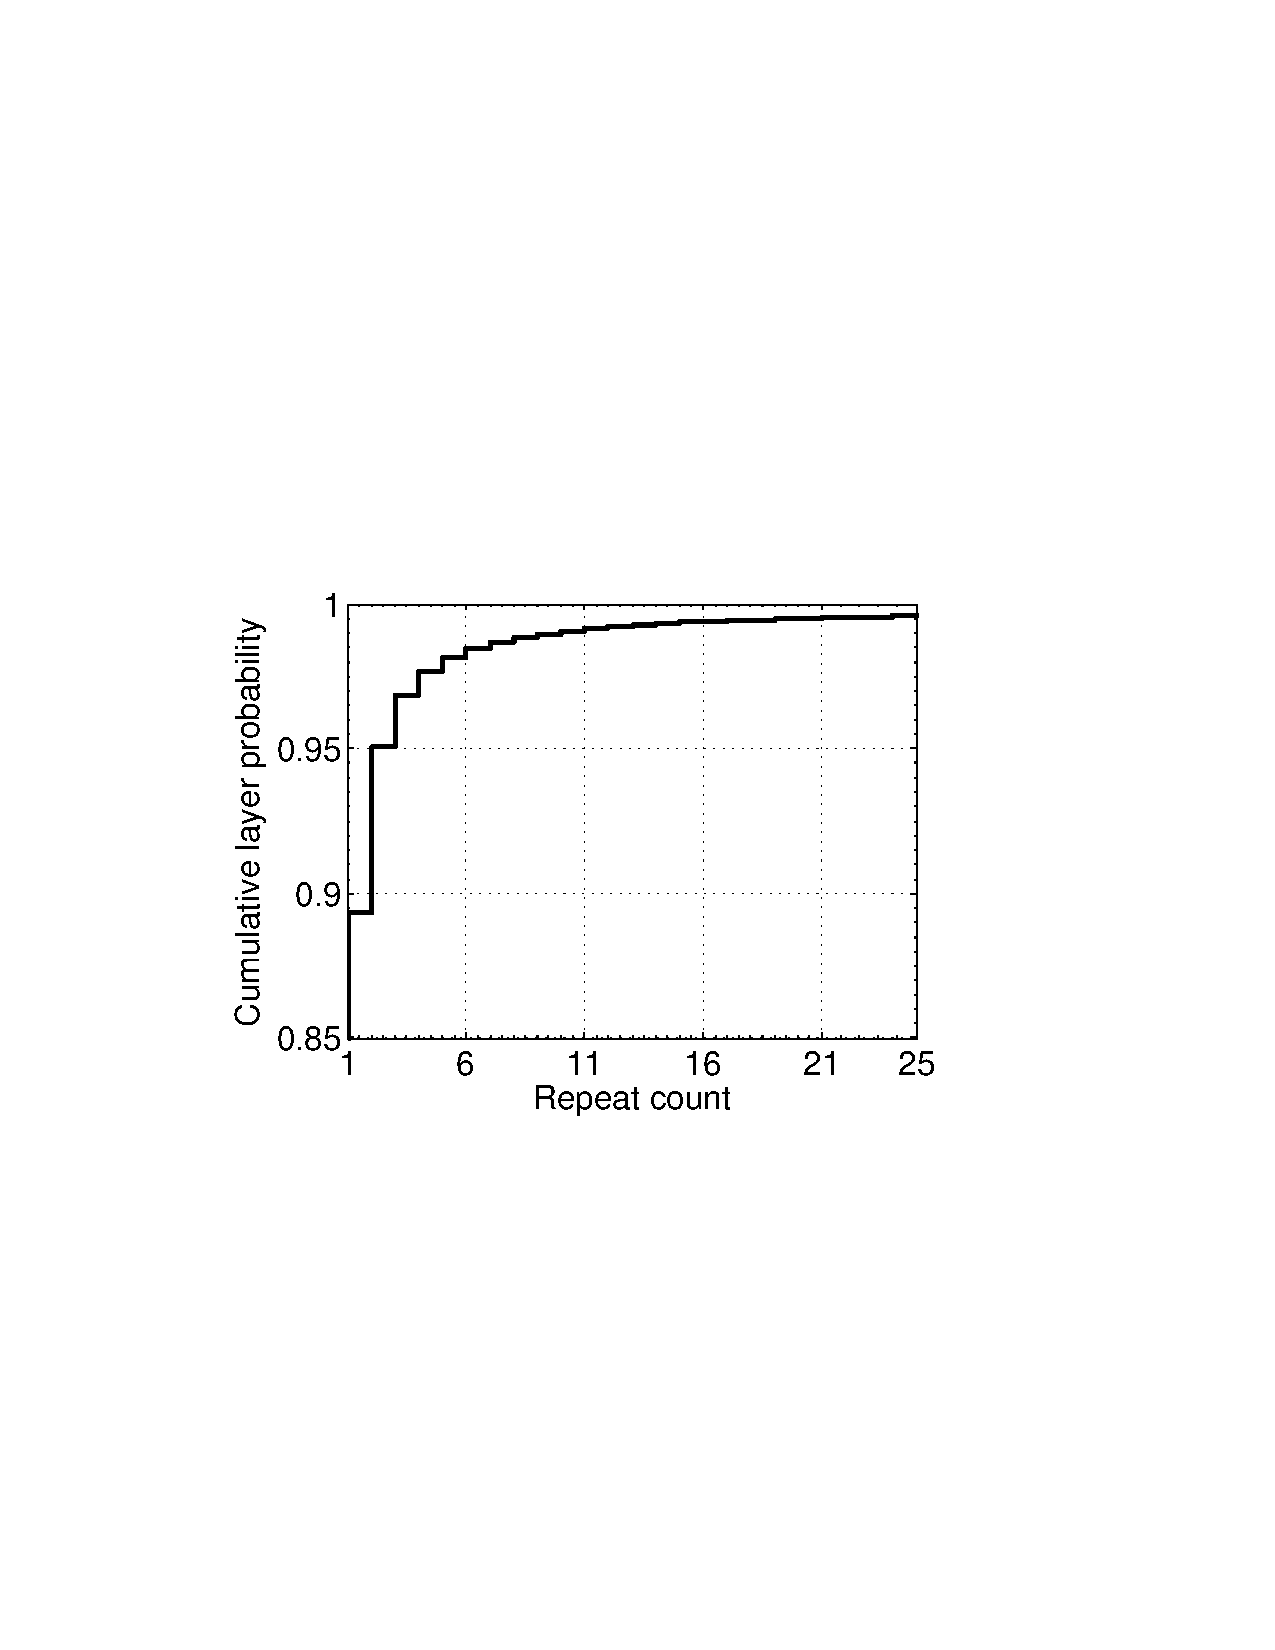
\includegraphics[width=0.23\textwidth]{graphs/repeate_layer.pdf}
	}
	\subfigure[Histogram of layer reference count]{\label{fig_hist_repeate_layer}
		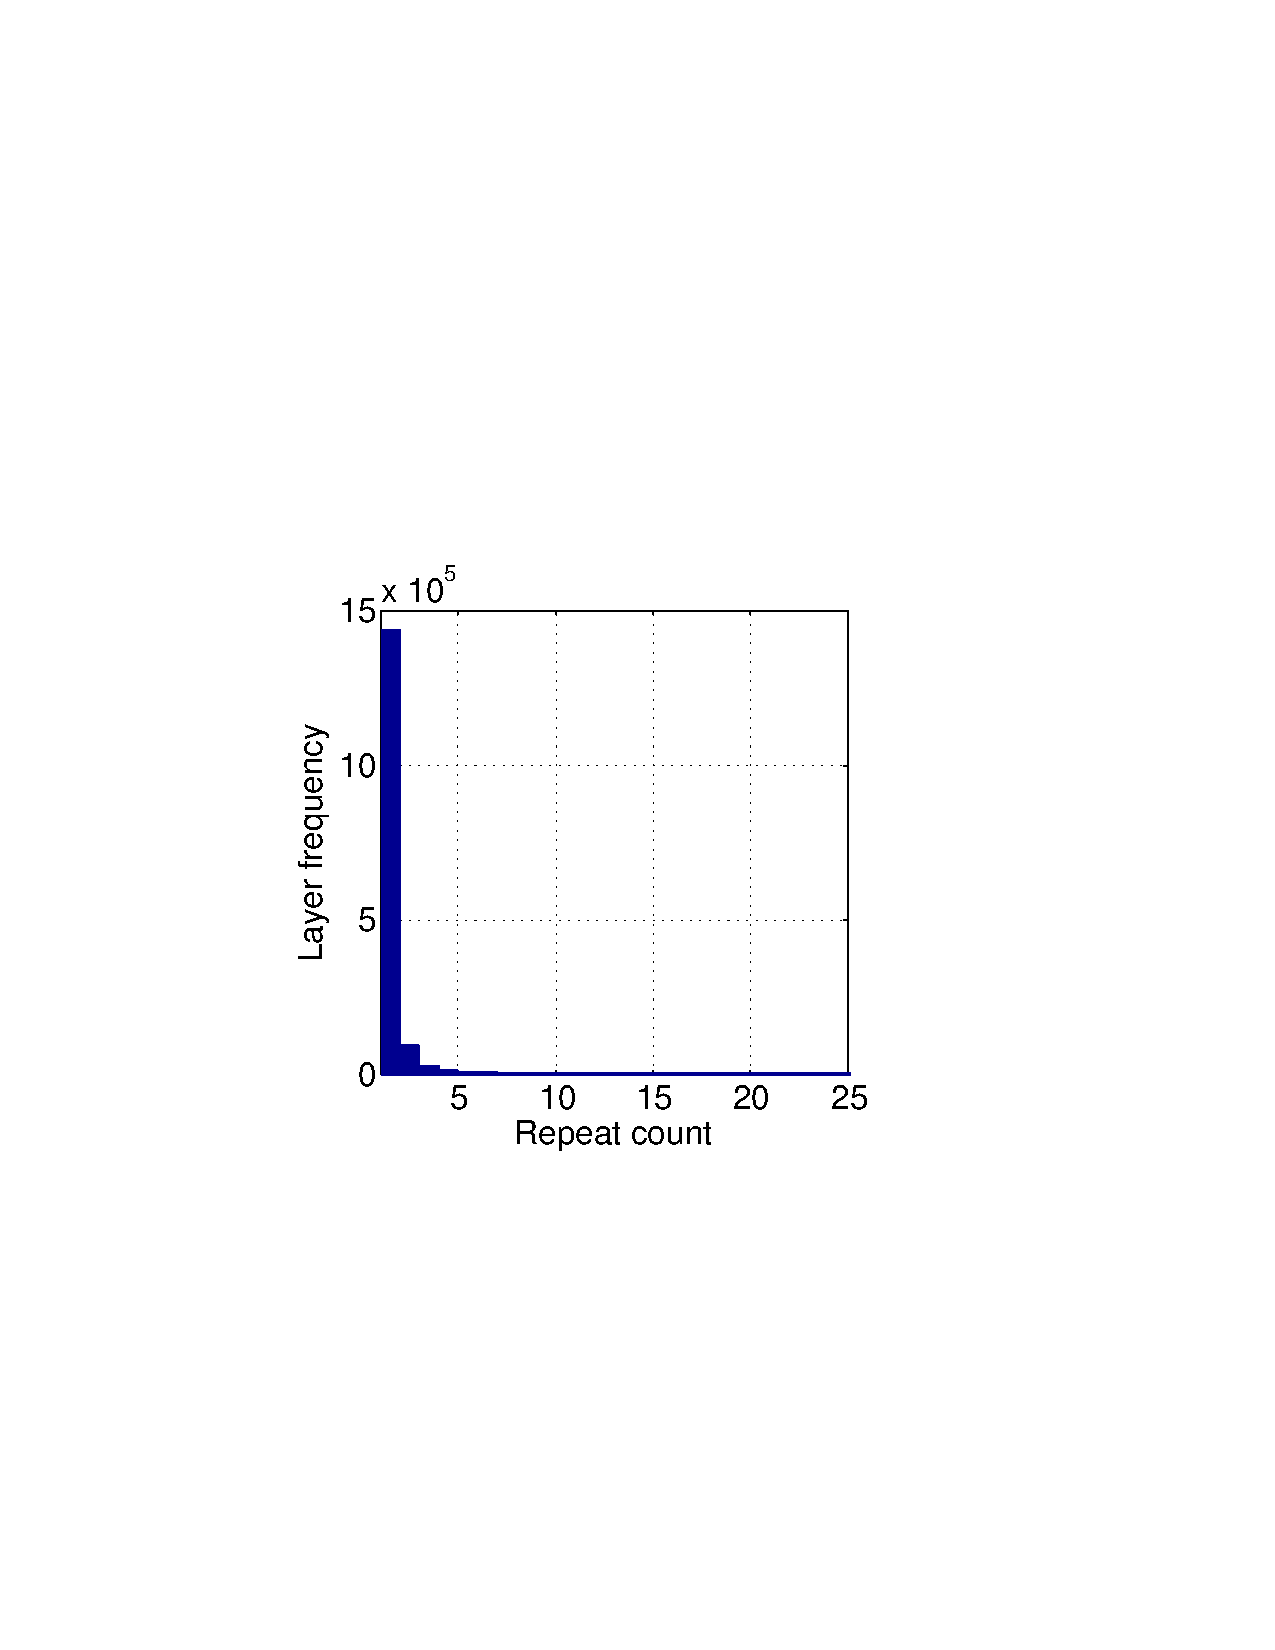
\includegraphics[width=0.223\textwidth]{graphs/hist_repeate_layer.pdf}
	}
	\caption{Layer reference counts across all images}
	\label{fig-repeat-layer-cnt}
\end{figure}

%\paragraph{Repeat layer count distribution}

An interesting question is what is the sharing rate of layers across images.
We analyze all image manifests and count for each layer, how many times it
is referenced by an image. Figure~\ref{fig_repeate_layer} shows that around 90\%
of layers are only reference by a single image while 95\% are reference by not
more than 2 images.
%99\% of layers are shared among less than 25 images. 
%
Figure~\ref{fig_hist_repeate_layer} shows the absolute values, revealing that
almost 1.5 million images are only referenced once. While there is again a large
spectrum of reference counts, the maximum is 33,428, the vast majority of layers
is not shared. This hints that the layer-based approach to improve storage
efficiency is barely utilized and there is room for improvement in how images
are constructed.


%%%%%%%%%%%%%%%%%%%%%%%%%%%%%%%%%%%%%%%%%%%%%%%%%%%%%%%%%%%%%%%%%%%%%


\paragraph{Directory and file count distribution}

\begin{figure}
	\centering
	\begin{minipage}{0.27\textwidth}
		\centering
		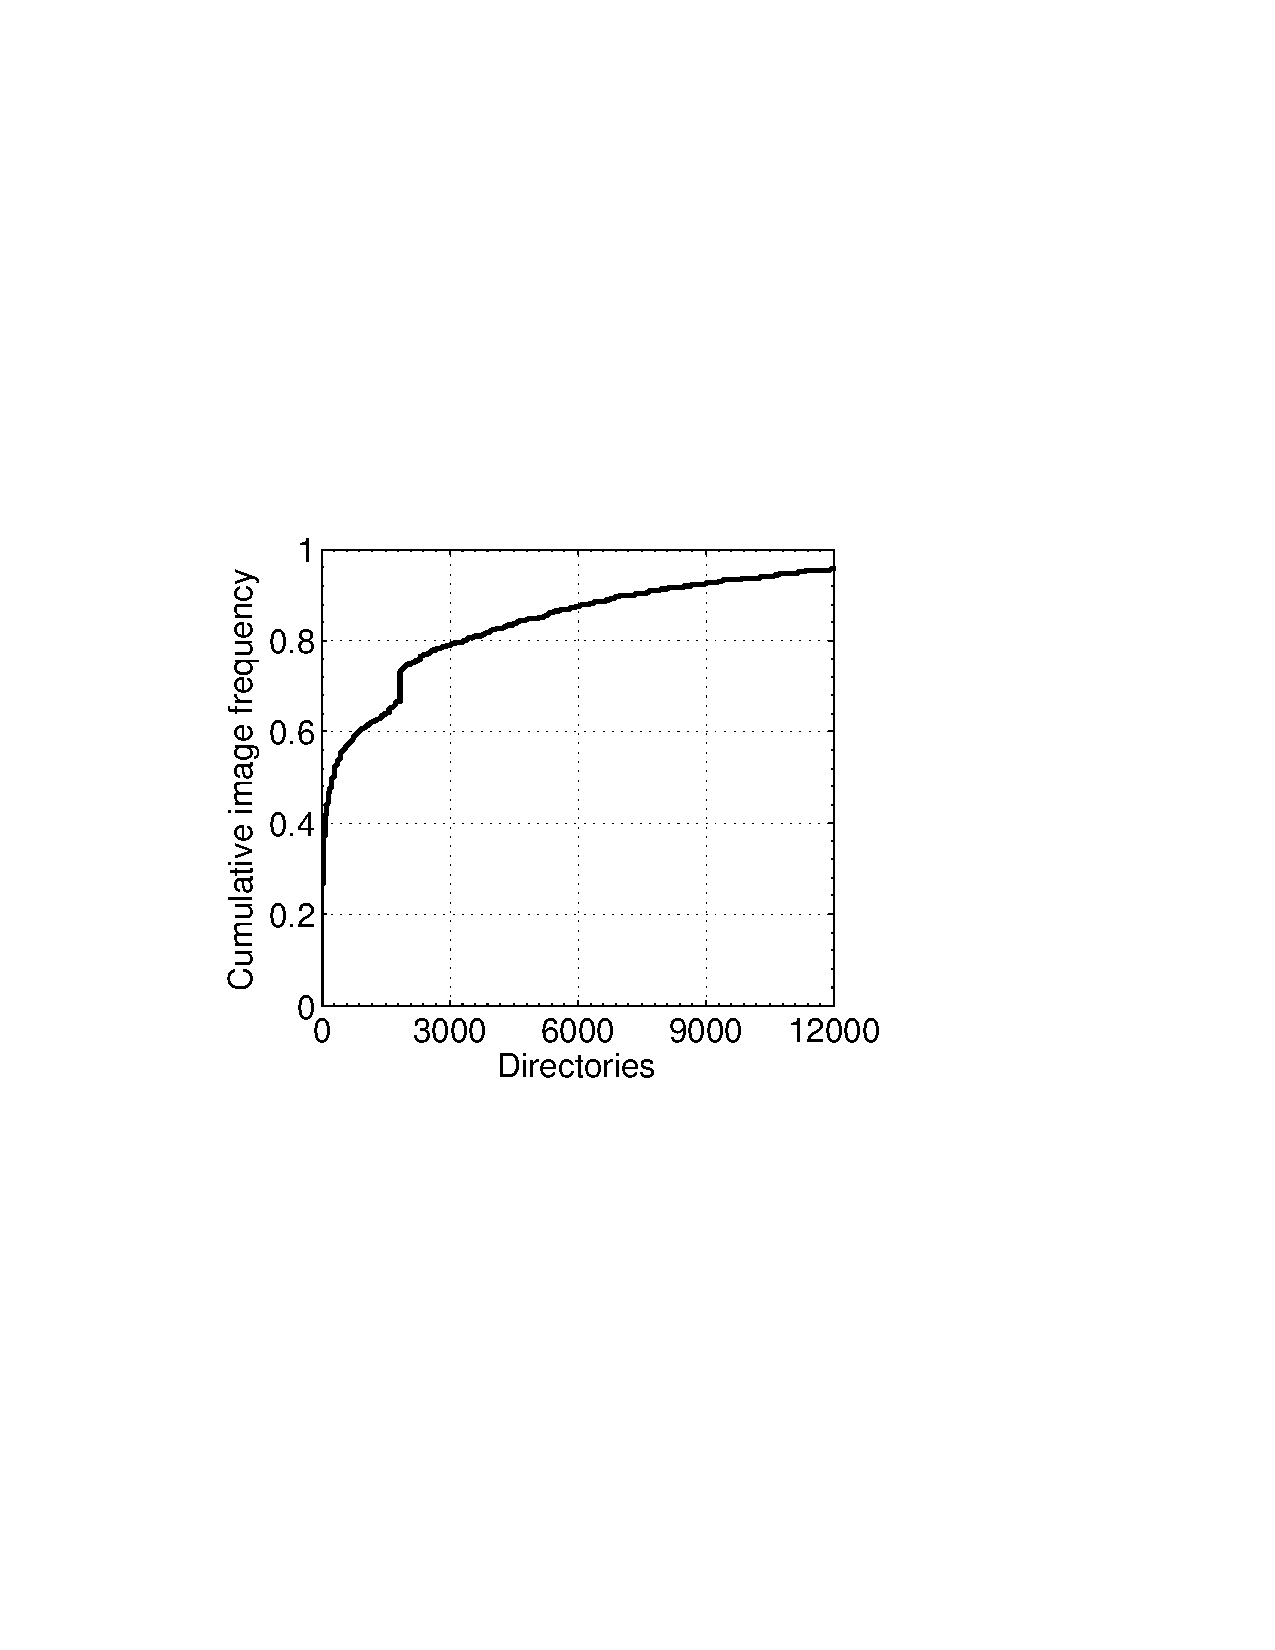
\includegraphics[width=1\textwidth]{graphs/dir.pdf}
		\caption{CDF of images by directories}
		\label{fig-dir}
	\end{minipage}%
	\begin{minipage}{0.23\textwidth}
		\centering
		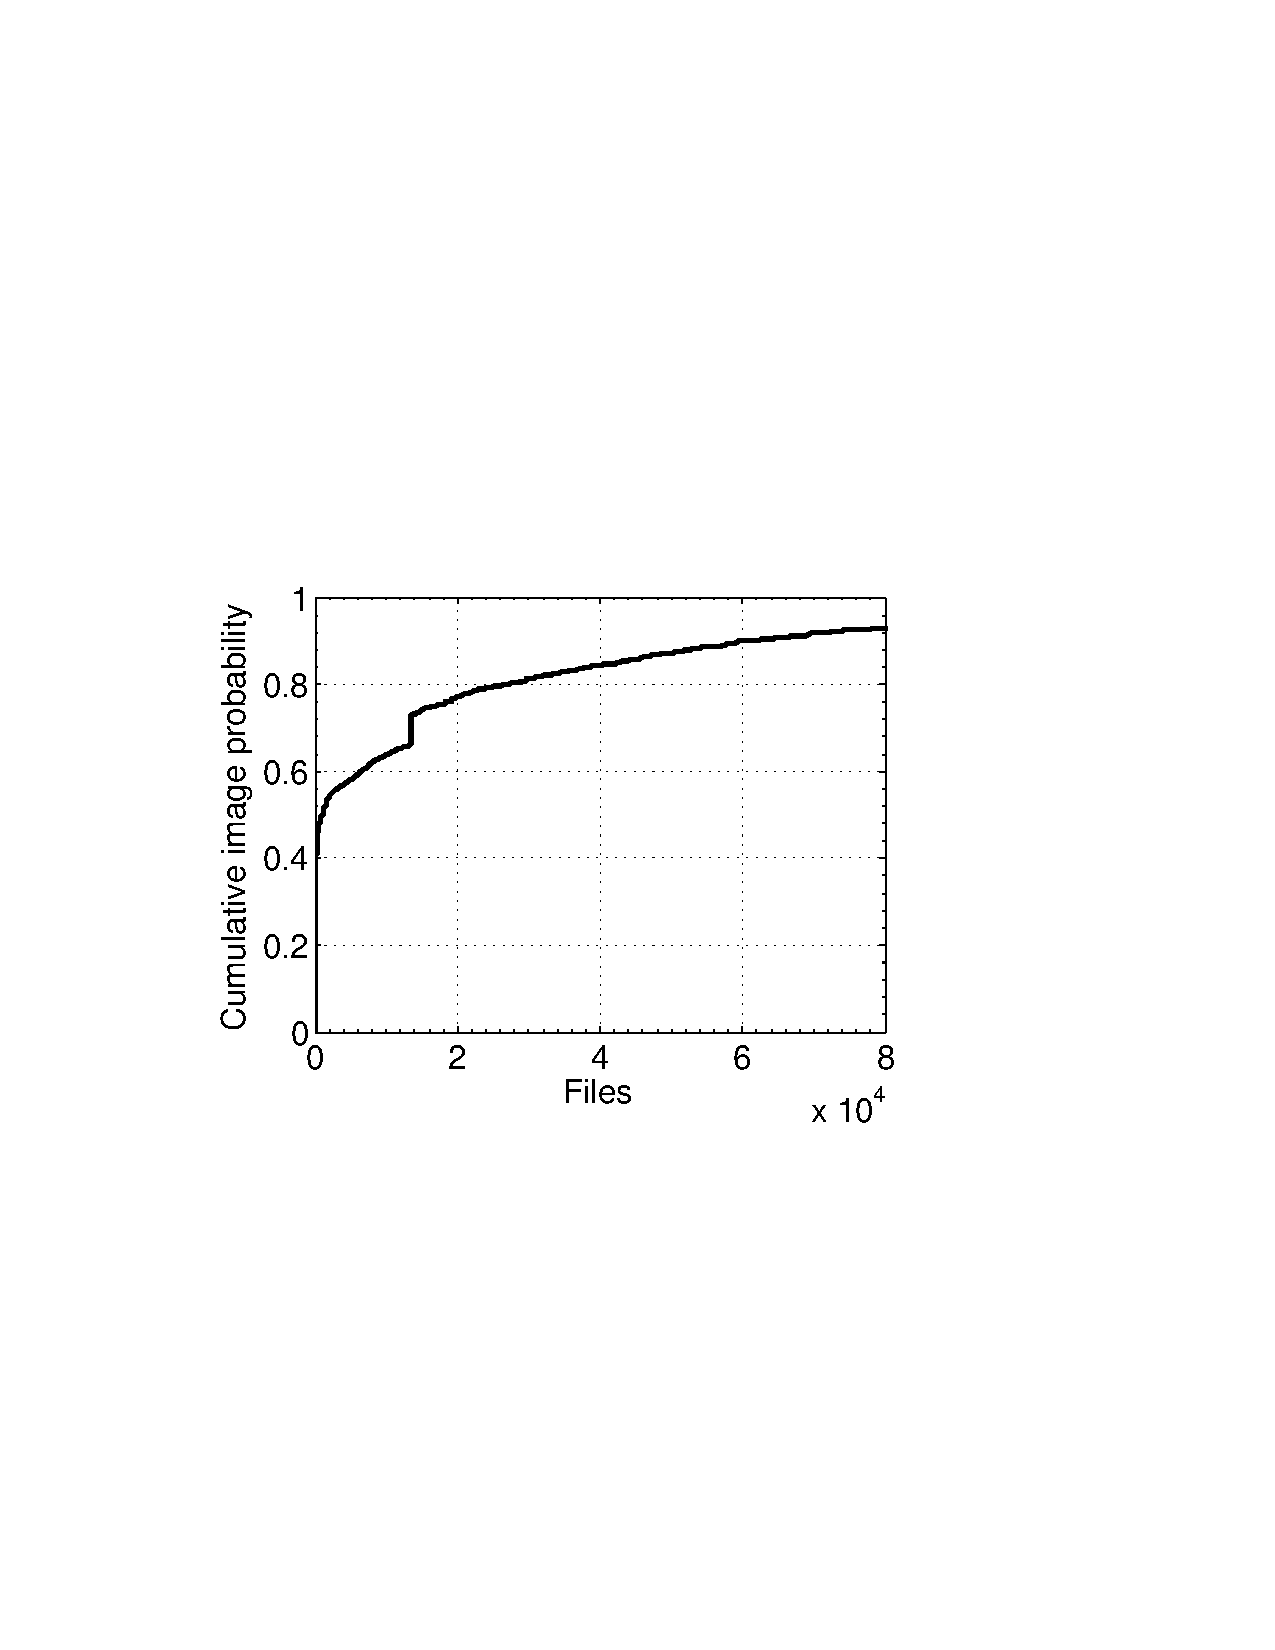
\includegraphics[width=1\textwidth]{graphs/file.pdf}
		\caption{CDF of images by files}
		\label{fig-file}
	\end{minipage}
\end{figure}

Lastly, we look at the directory (see Figure~\ref{fig-dir}) and file counts
(see Figure~\ref{fig-file}) in images to determine if deploying
images requires handling of large amounts of metadata. Looking at directories,
we see that 90\% of images have less than 7,344 directories while the median
is at 296. For files, 90\% of images have less than 64,780 files with a median
of 1,090.

This is consistent with our analysis of layer-based file and directory counts
and the number of layers per image. Again, we conclude that most images
do not require an extensive amount of metadata when being deployed as file and
directory counts are low except for few outliers.

%Figure~\ref{fig-dir} shows the cumulative image probability by directories. 90\% of images
%have less than 7,344 directories. Half of images have less than 296 directories. The maximum
%is 1,168,160 while the minimum is 1. The average is 2,705. 

%Figure~\ref{fig-file} shows the cumulative image frequency by files. 90\% of images have
%less than 64,780 files. Half of images have less than 1,090 files. The maximum is 8,509,958
%while the minimum is 1. The average is 21,413.
